\section{Teoría de la complejidad}
De manera empírica sabemos que existen problemas <<difíciles>> y problemas <<fáciles>>, por ejemplo, es mucho más difícil armar un rompecabezas que comprobar que está bien armado. La teoría de la complejidad busca responder a la pregunta: \textit{¿Qué hace a algunos problemas fáciles y a otros difíciles?} \cite{sipser1996introduction}. 

Uno de los logros de la teoría de la complejidad ha sido establecer un sistema de clasificación de acuerdo con la dificultad de los problemas. Este sistema consiste en muchas clases a las cuales puede ser asignado un problema en relación a los recursos computacionales necesarios para resolverlo, siendo las clases más estudiadas las que se definen por cantidad de operaciones (tiempo) y por memoria (espacio). 
A continuación se explica brevemente cómo se procede para describir la cantidad de operaciones necesarias para resolver un problema.

\subsection*{Notación gran $O$}
La cantidad de operaciones necesarias para resolver algún problema puede expresarse como una función del tamaño del mismo, es decir de la forma $f(n)$ donde $n$ es el tamaño del problema. La función $f$ puede ser de infinidad de formas diferentes, pero para fines prácticos solo se considera su comportamiento asintótico, es decir, cuando $n$ tiende a infinito. De esta manera se puede tener un conjunto de clases de equivalencia en las que se considera que los problemas tienen el mismo nivel de dificultad. Para delimitar estas clases se define la notación gran $O$.

Para dos funciones $f,g:\mathbb{R}\rightarrow\mathbb{R}$ se dice que $f(n)= O(g(n))$\footnote{El signo de igual aquí no tiene el sentido usual sino que más bien representa una relación entre conjuntos en la que $=$ quiere decir $\subseteq$ \cite{graham1989concrete}} si existen constantes $c,n_0\in\mathbb{R}^+$ tal que $0\leq f(n)\leq cg(n)$ para todo $n\geq n_0$ \cite{cormen2009introduction}.

De manera intuitiva $f(n)=O(g(n))$ quiere decir que $cg(n)$ es una cota superior a $f(n)$ como puede verse en la figura \ref{fig:bigo}.
\begin{figure}[H]
    \centering
    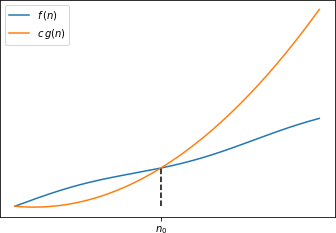
\includegraphics[scale=.8]{Imagenes/bigo.png}
    \caption{Representación de $f(n)= O(g(n))$}
    \label{fig:bigo}
\end{figure}
Se dice que un algoritmo es $O(g(n))$ si el número de operaciones que requiere para resolver un problema de tamaño $n$ es $O(g(n))$. Por ejemplo el algoritmo para sumar dos números de $n$ dígitos toma $O(n)$ operaciones. 

\subsection*{Clases \textbf{P} y \textbf{NP}}
La forma de la función $g$ es la base para clasificar los problemas de acuerdo a su complejidad. Dos de las clases más analizadas son definidas por el número de operaciones y se conocen como:
\begin{itemize} 
    \item \textbf{P}    Los problemas para los que se conoce un algoritmo para resolverlos que toma a lo más $Kn^c$ operaciones con $K,c$ finitas. El nombre de esta clase hace referencia que pueden resolverse en tiempo polinomial es decir que toman $O(n^c)$ operaciones para alguna $c$ positiva y finita. 
    \item \textbf{NP}   Los problemas para los que se puede verificar que se encontró una solución en tiempo polinomial. \footnote{Una definición alternativa pero equivalente se basa en el concepto de máquinas de turing no deterministas.}
\end{itemize}

Una subclase importante de la clase \textbf{NP} es la llamada \textbf{NP-completo} que incluye a los problemas para los cuales hallar un algoritmo de solución en tiempo polinomial implica hallar uno para todos los problemas en \textbf{NP}. De modo intuitivo es el conjunto de los problemas más difíciles en la clase.

Claramente \textbf{P} $\subseteq$ \textbf{NP}\footnote{Si ya tenemos un algoritmo que resuelve un problema en tiempo polinomial, para verificar si una solución es correcta solo hay que resolver el problema} pero determinar si también se cumple esta relación en sentido contrario, es decir determinar si \textbf{P} = \textbf{NP}, es un problema sumamente difícil con implicaciones importantes que no parece estar cerca de ser resuelto.

La distinción en algoritmos que toman tiempo polinomial parece arbitraria aunque de manera empírica se conocen muchos problemas de interés que pueden ser clasificados con esta definición. De un punto de vista más formal, los polinomios ejemplifican funciones de crecimiento lento y cumplen con varias propiedades teóricas que simplifican la clasificación de los problemas\cite{wigderson2006p}.


Muchos problemas de optimización de gran interés pertenecen a la clase \textbf{NP} entre ellos el JSP que se aborda que se aborda en el presente trabajo y que en particular es \textbf{NP-completo}. Ante la dificultad para resolver estos problemas de manera eficiente surgieron técnicas conocidas como metaheurísticas que buscan facilitar encontrar soluciones aceptables aunque no óptimas.


